\documentclass[final]{beamer}

\usepackage[T1]{fontenc}
 \usepackage[utf8]{luainputenc}
\usepackage{lmodern}
\usepackage[size=custom, width=122,height=91, scale=1.2]{beamerposter}
\usetheme{gemini}
\usecolortheme{bgu}
\usepackage{graphicx}
\usepackage{booktabs}
\usepackage{tikz}
\usepackage{pgfplots}
\pgfplotsset{compat=1.14}
%\usepackage{anyfontsize}


\newlength{\sepwidth}
\newlength{\colwidth}
\setlength{\sepwidth}{0.025\paperwidth}
\setlength{\colwidth}{0.3\paperwidth}

\newcommand{\separatorcolumn}{\begin{column}{\sepwidth}\end{column}}



\title{Rubik's Mathematics: A Twist on Numbers}

\author{Jeremy Huang and Benedict Antonious}

\institute[shortinst]{University of Colorado Boulder}



\logoleft{
\includegraphics[height=4.5cm]{logos/BoulderLogo.png}}


\begin{document}

\begin{frame}[t]
\begin{columns}[t]
\separatorcolumn

\begin{column}{\colwidth}

  \begin{block}{Abstract}
    \large The Rubik's Cube, an iconic 3D puzzle, has captured the imagination of enthusiasts and mathematicians alike for decades. This poster delves into the mathematical intricacies of the Rubik's Cube. We investigate the cube's symmetry, its staggering number of possible permutations, and the use of computer aided proof-assistants to calculate the algorithms to solve the Rubik's Cube. Whether you're a puzzle enthusiast or a math fanatic, this poster invites you to embark on a fascinating journey into the world of Rubik's Cube mathematics.


  \end{block}

  \begin{block}{Combinations of a Rubik's Cube}

    \large There are three (four if you count the not-visible core) types of pieces:

    \begin{itemize} %Talk about centers/edges/corners
      \item \textbf{Corners:} 8 of these on each corner of the cube
      \item \textbf{Edges:} 12 of these connecting adjacent corners
      \item \textbf{Centers:} 6 of these on each face of the cube
    \end{itemize}

    There are $8!$ ways we can permute the corner pieces to the corners of a cube, and $12!$ ways 
    we can permute the edge pieces into the 12 edge slots of a cube. There are $3^8$ ways we can orient 
    the corner pieces and $2^{12}$ ways we can the edge pieces. We also have to divide by $12$, 
    since some states are impossible. This yields the final formula: \\

    $$ \displaystyle\frac{8!\cdot 12! \cdot 3^8 \cdot 2^{12}}{12} = 43252003274489856000 $$ \\

    \begin{figure}
      \centering
                    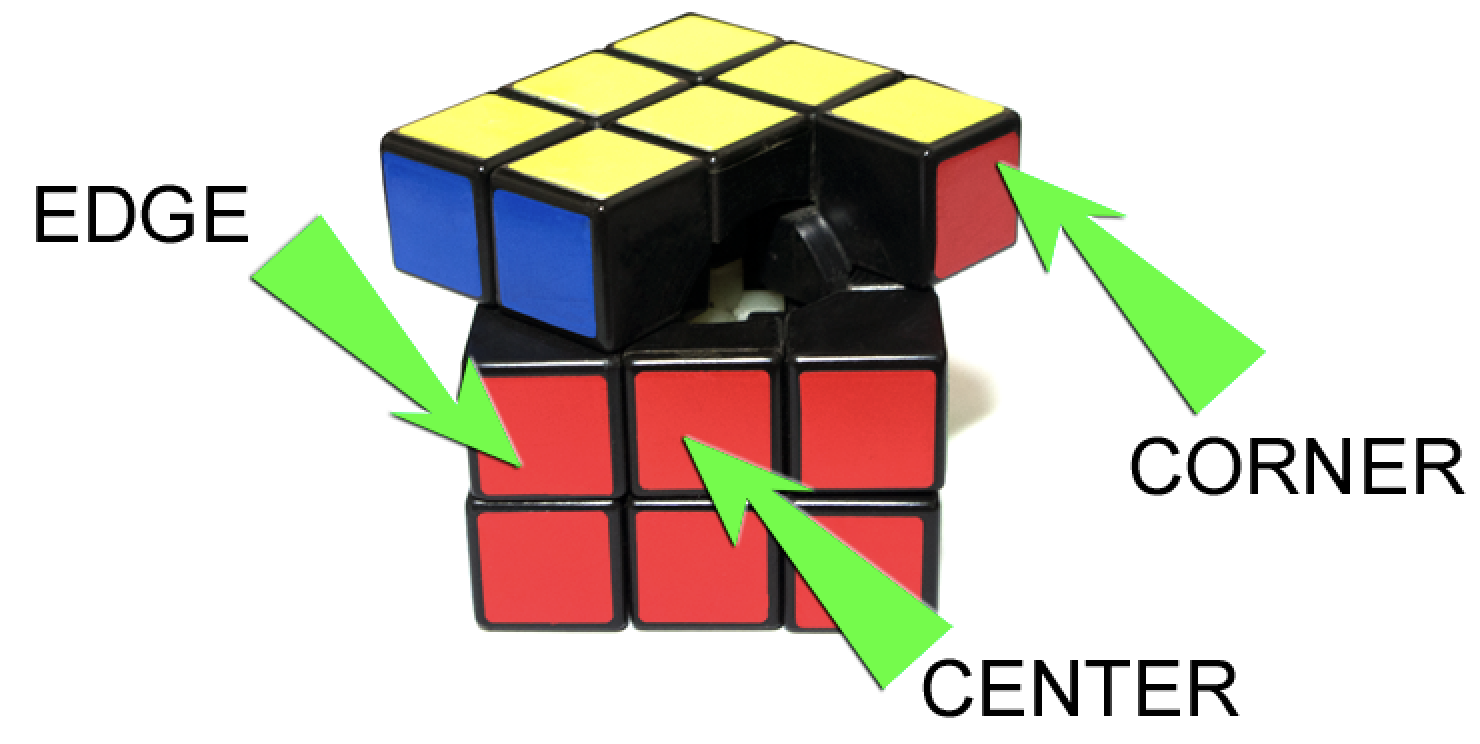
\includegraphics[width=0.6\textwidth]{logos/rubikspieces.png}
    \end{figure}

  \end{block}

  \begin{block}{How big is 43 Quintillion?}

    \large 
    %Imagine we find a new, unique Rubik's cube combination every second. There are
    %about 31 million seconds in a year, so it would take more than 1.3 trillion years. \\
    %Imagine we started doing this during the Dinosaur Age: we would only get to 2 quadrillion combinations. \\
    %We would have to repeat the process more than 20,000 times to reach all 43 quintillion combinations! \\
    Imagine we had a dollar for each rubik's cube combination there was. If were to lay one layer of one dollar bills in
    Colorado, it would take 25 trillion dollars. We would have to stack that another 2 million times to use all of our money. \\
    The stack would be about the same height of the tallest building in Denver. In other words,
    the money would cover all of Colorado in a layer as tall as a skyscraper.
    \begin{figure}
      \centering
                    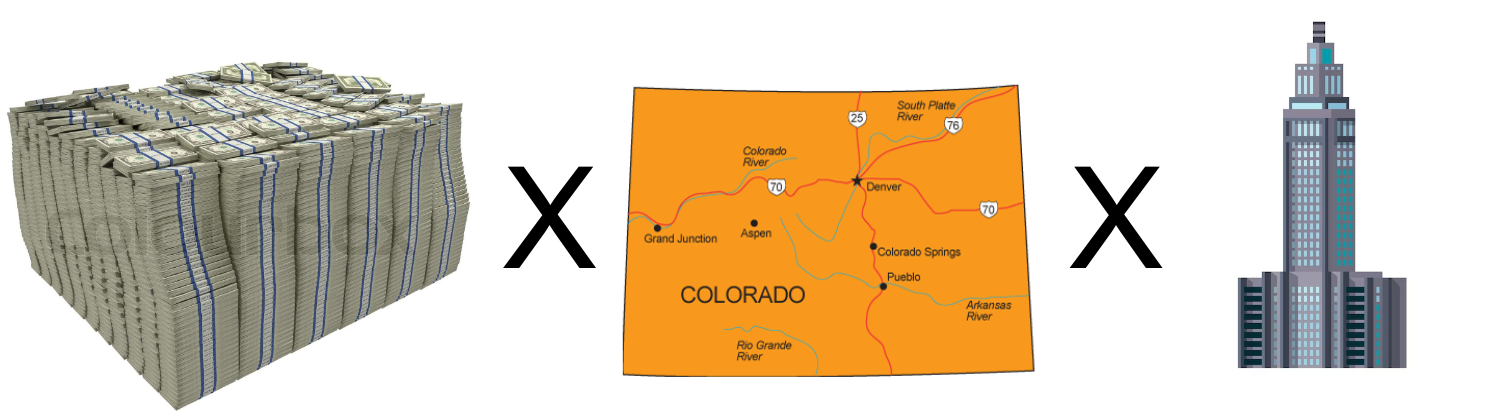
\includegraphics[width=0.9\textwidth]{logos/moneyvisual.png}
    \end{figure}

  \end{block}

\end{column}

\separatorcolumn

\begin{column}{\colwidth}

  \begin{block}{Solving a Rubik's Cube}

    \large VA popular method for speed-solving is CFOP(used by many world record holders) where you create a Center \textbf{Cross}, solve the First two layers(\textbf{F2L}), Orient the last layer(\textbf{OLL}), and Permute the last layer(\textbf{PLL}). 
    We can figure out the maximum number of moves it would take for a solve using CFOP by going adding up the maximum steps of each step: 
    \begin{enumerate}
      \item For the center cross, the maximum needed is eight
      \item For F2L, it depends but the maximum is around 24-28
      \item For OLL, we can get a maximum of 11
      \item And finally for PLL, the maximum is 14
    \end{enumerate}
    Across the four steps in CFOP we have about 60 moves needed to solve a 3x3 Cube.

  \end{block}

  \begin{block}{God's Algorithm and Number}

    \large Naturally, people want to know how to solve the know the best ways to solve
    a Rubik's cube. \textbf{God's algorithm} refers to the hypothetical perfect solving 
    method for a Rubik's Cube, a sequence of moves that would guarantee the shortest possible 
    solution for any scrambled configuration. \textbf{God's number} represents the maximum 
    number of moves required to solve the most challenging possible Rubik's Cube configuration. 
    This value was proven to be 20 in July 2010 after extensive computer-assisted calculations 
    and mathematical research, providing a fundamental benchmark for the cube's complexity.
    \begin{center}
    \begin{tikzpicture}[scale=1.13]
      \begin{axis}[xtick = {12,13,14,15,16,17,18,19,20},
          ymin=0, ymax=100, xmin = 12, xmax = 21, xlabel = \# of moves,
          area style, width=25cm,height=9cm, xticklabel style = {xshift=1.3cm}
          ]
        \tikzstyle{every node}=[font=\small]
      \addplot+[ybar interval,mark=no] plot coordinates { (0, 0) (1, 0) (2, 0) (3, 0) (4,0) (5,0) (6,0)
       (7,0) (8,0) (9,0) (10,0) (11,0) (12,0) (13,0) (14,0) (15, 0.2) (16, 2.5) (17, 27.7) (18, 67) (19, 3.5) (20,0) (21,0) };
        \node[] at (axis cs: 16.5,10) {2.5\%};
        \node[] at (axis cs: 17.5,36) {27.7\%};
        \node[] at (axis cs: 18.5,76) {67\%};
        \node[] at (axis cs: 19.5,12) {3.5\%};
        \node[] at (axis cs: 20.5, 10) {<0.1\%};
        \node[] at (axis cs: 14, 9) {<0.1\%};

      \end{axis}
      \end{tikzpicture}
    \end{center}

  \end{block}

  \begin{block}{Proof Assistants/Computer Aided proof}

    \large Obviously, it would be impossible for humans to go through all 43 Quintillion
    combinations of a Rubik's cube. However, computers have been able to use exhaustive search
    and other techniques to determine God's number. Other proofs that have used computers include:

    \begin{itemize}
      \item \textbf{Connect Four:} Proved the game is deterministic
      \item \textbf{Kepler's Conjecture:} Optimal sphere-packing in 3 Dimensions
      \item \textbf{Sudoku:} You need at least 12 clues to solve a Sudoku Puzzle
    \end{itemize}

  \end{block}

\end{column}

\separatorcolumn

\begin{column}{\colwidth}

  \begin{block}{Applications to Speed Cubing}

    \large There are many different methods for Speed Cubing, all aimed at Solving
    the cube as fast as possible. This involves coming up with ways to use
    less moves and using easily executed algorithms. Here are a couple:

    \begin{table}
      \centering
      \begin{tabular}{l r r c}
        \toprule
        \textbf{Method} & \textbf{\# Turns} & \textbf{\# Algorithms} & \textbf{Average Times (s)} \\
        \midrule
        Beginner & 80-100 & 15 & 30-120 \\
        CFOP & 55-60 & 78 & 5-30 \\
        Roux & 45-50 & 100+ & 5-20 \\
        ZZ & 45-55 & 493 & 5-15 \\
        \bottomrule
      \end{tabular}
    \end{table}


  As more methods and algorithms get developed with the aid of computers,
  speed-cube times have been getting lower considerably:

  \begin{figure}
    \centering
      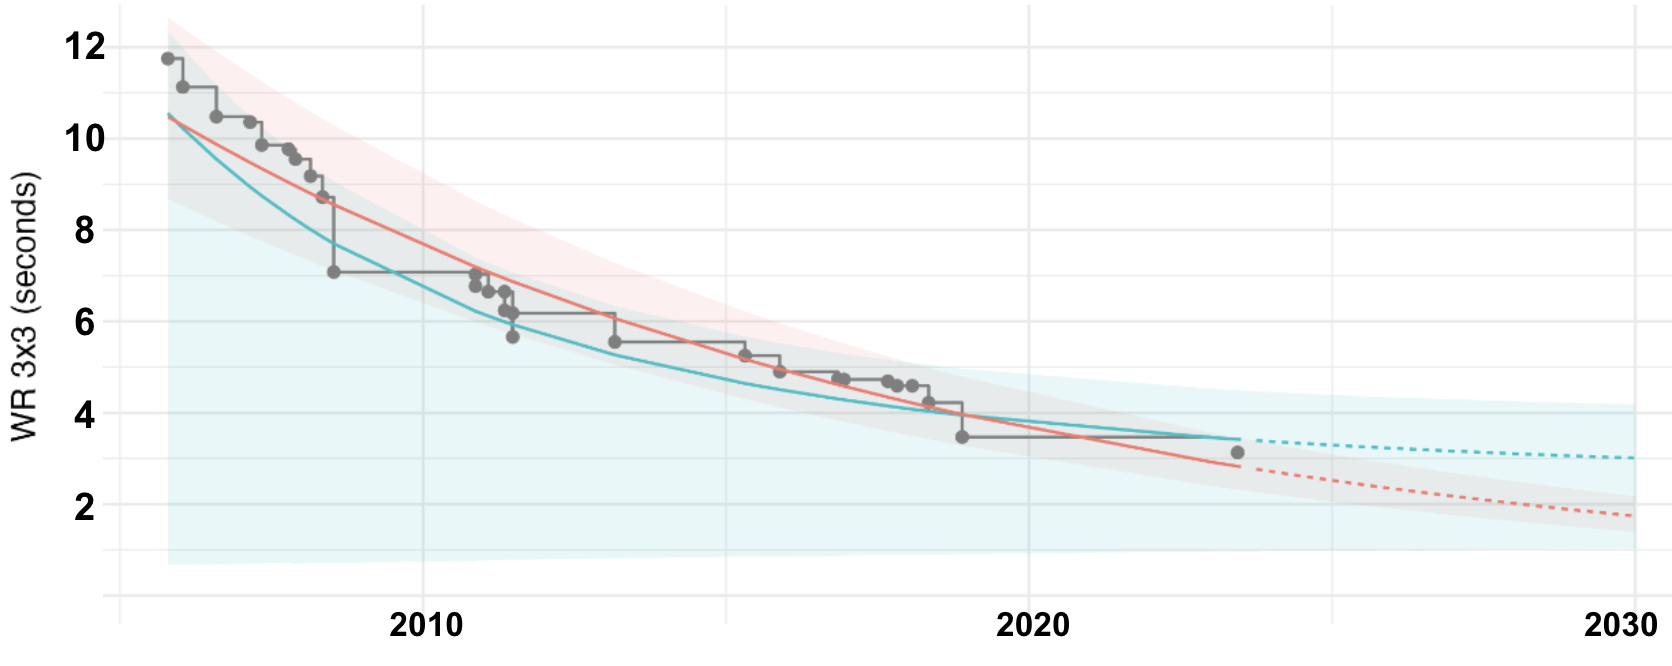
\includegraphics[width=1.0\textwidth]{logos/solveprogression.png}
  \end{figure}

  \end{block}

  \begin{block}{What about larger Rubik's Cubes?}
    
    \large Unsurprisingly, the number of possible combinations of larger Rubik's Cube scale exponentially \\
    
    \begin{itemize}
      \item \textbf{4x4:} 7.4 quattuordecillion ($7.5\cdot 10^{45}$) - 20s solve time
      \item \textbf{5x5:} 283 trevigintillion ($283 \cdot 10^{72}$) - 38s solve time
      \item \textbf{6x6:} Big number with 117 digits - 75s solve time
      \item \textbf{7x7:} Big number with 165 digits - 110s solve time
    \end{itemize}

    The general formula for the combinations on an $n \times n$ cube is: \\

    $$ \displaystyle 7! \cdot  3^6 \left( 24 \cdot 2^{10} \cdot 12!  \right)^{n \text{ mod} 2}
    (24!)^{\lfloor \frac{n-2}{2} \rfloor} \left( \displaystyle\frac{24!}{4!^{6}} 
    \right)^{\lfloor \left( \frac{n-2}{2} \right)^2 \rfloor} $$ \\


  \end{block}

  \begin{block}{References}

    \nocite{*}
    \footnotesize{\bibliographystyle{plain}\bibliography{poster}}
    \begin{enumerate}
    \item God’s number is 20 (2021) God’s Number is 20. Available at: https://www.cube20.org/.\\[0.1cm]
    \item kaixax555 (2013) Structure of a Rubik’s Cube, Cube Observatory. Available at: https://cubeobservatory.wordpress.com/2013/07/28/structure-of-a-rubiks-cube/.  \\[0.1cm]
    \item Online nxnxn rubik’s cube simulator (2021) Ruwix. Available at: https://ruwix.com/blog/nxnxn-cube-simulator-solver/.  \\[0.1cm]
    \item Winslow, A. (2011) Algorithms for solving Rubik’s Cubes, arXiv.org. Available at: https://arxiv.org/abs/1106.5736/.  \\[0.1cm]
    \item Nguyen, M. (2020) How Close Are Computers to Automating Mathematical Reasoning?. Available at: https://www.quantamagazine.org/how-close-are-computers-to-automating-mathematical-reasoning-20200827/ \\[0.1cm]
    \item Speedcubing (2023) Wikipedia. Available at: https://en.wikipedia.org/wiki/Speedcubing. \\[0.1cm] 
    \item R/cubers (2019) Reddit. Available at: https://www.reddit.com/r/Cubers/. 
    \end{enumerate}
  \end{block}

\end{column}

\separatorcolumn
\end{columns}
\end{frame}

\end{document}
